% ---------------------------- README -----------------------------------------
% This file holds section four of the body of the Machine Intelligence II 
% script.
% -----------------------------------------------------------------------------

\setcounter{equation}{0}
\newpage 
\section{Clustering and Embedding}

While projection methods search for interesting directions / features
along which data differ, clustering methods yield groupings of the
data according to a specified similarity or distance measure.

While methods of central clustering typically also find
representatives (e.g.\ group averages or prototypes) for these different groups,
\emph{pairwise clustering} methods just need estimates of distances
(e.g. similiarity judgements) between pairs of data points. 
% -----------------------------------------------------------------------------

\subsection{K-means Clustering}

% -----------------------------------------------------------------------------

\subsubsection{The Clustering Problem}
\paragraph{Goal:} partitioning of observations 
$\vec{x}^{(\alpha)}, \alpha = 1, \ldots, p; \vec{x}^{(\alpha)} \in \mathbb{R}^N$
according to similarity. This is illustrated in figure \ref{fig:clusteringProblem}. 
\begin{figure}[h!]
  \centering
  \includegraphics[width=10cm]{section4_fig1}  
  \caption{The clustering problem}
  \label{fig:clusteringProblem}
\end{figure}

\begin{itemize}
	\itR unsupervised formation of categories (partitions, clusters) 
		according to predefined criteria
	\itR description of clusters by prototypes $\leftarrow$ ''central'' 
		clustering
\end{itemize}


\paragraph{K-means Clustering:} ``prototype-based clustering''
\label{sec:kmeans}
\begin{itemize}
\item based on average quadratic Euclidean distance between observations and prototypes
\item simple \& most common procedure for clustering of vectorial data
\end{itemize}
\textbf{Cluster model:}\\\\
prototypes: $\vec{w}_q, q = 1, \ldots, M$ \qquad\qquad (M: number of clusters)
\\\\
binary assignment variables $m_q^{\alpha}$:
\begin{equation}
	m_q^{(\alpha)} = \left\{ \begin{array}{ll}
		1, & \text{if } \vec{x}^{(\alpha)} \text{ belongs to cluster } q
		\\\\
		0, & \text{else}
	\end{array} \right. 
\end{equation}
normalization:
\begin{equation}
	\sum\limits_q m_q^{(\alpha)} = 1
\end{equation}
cost function (''empirical risk''):
\begin{equation}\label{eq:euclideanClusterCost}
	E_{ \big[ \big\{ m_q^{(\alpha)} \big\}, \big\{ \vec{w}_q \big\} 
		\big] }^T = \frac{1}{2p} \sum\limits_{q,\alpha} m_q^{(\alpha)}
		\big( \vec{x}^{(\alpha)} - \vec{w}_q \big)^2
\end{equation}
The cost function represents the average quadratic distance between
observations and prototypes (''variance''). The choice of
similarity/distance measure should be based on prior knowledge (if available). 

Remark: If $\vec{w}_q$ is center of mass $\implies$ $E^T = \frac{1}{2} \cdot \mathrm{variance}$.
\\\\
model selection:
\begin{equation}
	E^T \eqexcl \min \leftarrow \substack{	\text{continous/discrete} \\
						\text{optimization problem}}
\end{equation}
\[ \text{validation} \left\{ \begin{array}{c}
	\substack{	\text{no, if goal is ''just'' to} \\
			\text{describe the set of observations}} \\\\
	\substack{	\text{yes, if goal is inference/prediction} \\
			\text{on future observations (e.g. calculating} \\
			m_q^{(\mathrm{new})} \text{ for a new observation }
			\vec{x}^{(\mathrm{new})} \text{)}}
\end{array} \right. \]
The computations involved in the cost function for k-means clustering are illustrated in figure \ref{fig:kMeansCostfunction}. 
\begin{figure}[h!]
  \centering
\includegraphics[width=10cm]{section4_fig2}  
  \caption{Illustration of the k-means cost function}
  \label{fig:kMeansCostfunction}
\end{figure}



% -----------------------------------------------------------------------------

\subsubsection{Model Selection}
\label{kmeans_modelselection}
Optimization problem with continuous (cluster-centers) and discrete
(cluster-assignment: binary) variables. Dissimilarity measure is Euclidean distance. 
\begin{itemize}
	\itR two step descent procedure (algorithm \ref{alg:batch-k-means})
\end{itemize}
\begin{algorithm}[h!]
\DontPrintSemicolon
  randomly initialize prototypes e.g.\ around (i.e., +noise) the whole data's center of mass, e.g., using PCA for spread quantification\;
  \Begin(loop){
  (1) choose  $m_q^{(\alpha)}$ ... \;
... such that $E^T$ is minimal for the given prototypes\;
\[ m_q^{(\alpha)} \left\{ \begin{array}{ll}
	1, & \text{if } q = \argmin_{\gamma} \big| \vec{x}^{(\alpha)}
		- \vec{w}_{\gamma} \big| \\
	0, & \text{else}
\end{array} \right. \]
$\Rightarrow$ assign every data point to its nearest prototype \;
\;
(2) choose  $\vec{w}_q$ ...\;
... such that $E^T$ is minimal for the -new- assignments\;
\[ \vec{w}_q = \frac{\sum\limits_{\alpha} m_q^{(\alpha)} \vec{x}^{(\alpha)}}{
	\sum\limits_{\alpha} m_q^{(\alpha)}}
\]
$\Rightarrow$ set $\vec{w}_q$ to the center of mass of its assigned data
}
    \label{alg:batch-k-means}
    \caption{batch k-means}
\end{algorithm}

\paragraph{center of mass is optimal:} condition for extremal point:
\begin{equation}
	\begin{array}{ll}
	\frac{\partial}{\partial \vec{w}_q} \bigg\{ \frac{1}{2p} 
	\sum\limits_{q^{'}, \alpha} m_{q^{'}}^{(\alpha)} 
	\big( \vec{x}^{(\alpha)} - \vec{w}_{q^{'}} \big)^2 \bigg\}
	& = -\frac{1}{p} \sum\limits_{\alpha} m_q^{(\alpha)} 
		\big( \vec{x}^{(\alpha)} - \vec{w}_q \big) \eqexcl 0 \\\\
	& \leadsto \vec{w}_q = \frac{\sum\limits_{\alpha} m_q^{(\alpha)}
		\vec{x}^{(\alpha)}}{\sum\limits_{\alpha} m_q^{(\alpha)}}
	\end{array}
\end{equation}
condition for minimum:
\begin{equation}
	\begin{array}{ll}
	\frac{\partial^2}{\partial \mathrm{w}_{qi} \partial \mathrm{w}_{
		q^{''}j}} \bigg\{ \frac{1}{2p} \sum\limits_{q^{'}, \alpha}
		m_{q^{'}}^{(\alpha)} \big( \vec{x}^{(\alpha)} - \vec{w}_{q^{'}}
		\big)^2 \bigg\} 
	& = \frac{\partial}{\partial \mathrm{w}_{q^{''}j}} \bigg\{
		-\frac{1}{p} \sum\limits_{\alpha} m_q^{(\alpha)} 
		\big( \mathrm{x}_i^{(\alpha)} - \vec{w}_{qi}
		\big) \bigg\} \\\\
	& = \Big( \frac{1}{p} \sum\limits_{\alpha} m_q^{(\alpha)} \Big)
		\delta_{ij} \delta_{qq^{''}}
	\end{array}
\end{equation}
\begin{itemize}
	\itl diagonal matrix with all positive entries
	\itl condition for minimum always fulfilled
\end{itemize}
\begin{itemize}
\item $E^T$ is non-increasing in every step and $E^T$ is bounded from below $\Rightarrow$ K-means clustering converges to a (local) optimum of $E^T$. 
\item $E^T$ at the solution can be interpreted as the average variability
within the groups.
\end{itemize}
\begin{figure}[h!]
  \centering
  \includegraphics[width=9cm]{section4_fig3}  
  \caption{k-means and tesselation}
  \label{fig:tesselation}
\end{figure}


tesselation cell: region of data space for which
\begin{equation}
	q = \argmin_{\gamma} \big| \vec{x} - \vec{w}_{\gamma} \big|
\end{equation}
This interpretation is illustrated in figure \ref{fig:tesselation} and provides an alternative 2-step interpretation of k-means clustering
in terms of an optimized tesselation of the input-space:
\begin{enumerate}[(1)]
\item construct tesselation of feature space
\item adjust prototypes to the center of mass of all data points 
		within the corresponding tesselation cell
\end{enumerate}

\paragraph{''on-line'' version of K-means Clustering:}
The k-means procedure can be implemented in an on-line fashion (algorithm \ref{alg:on-line-k-means}) that is often more robust wrt.\ local minima than batch-learning and can be useful for streaming-data. 
\begin{algorithm}[h]
  \DontPrintSemicolon
  initialize prototypes e.g.\ around center of mass \;
  select learning step  $0 < \eta << 1$\;
  \Begin(loop){
    choose a data point $\vec{x}^{(\alpha)}$ \;
    assign data point to its closest prototype $q$\;
    \[ q = \argmin_{\gamma} \big| \vec{x}^{(\alpha)} - \vec{w}_{\gamma} \big| \]
    change corresponding prototype according to\;
    \[ \Delta \vec{w}_q = \eta \big( \vec{x}^{(\alpha)} - \vec{w}_{\gamma} \big) \]
    change $\eta$ \;
  }
  \label{alg:on-line-k-means}
  \caption{on-line k-means}
\end{algorithm}
\\
Goodness of the found solution depends on choosing an appropriate ''annealing'' schedule for $\eta$: Robbins-Monro conditions ({\it cf. MI I, section 1.4.1}). A typical schedule is shown in figure \ref{fig:annealingScheduleKMeans}. 
\begin{figure}[h!]
  \centering
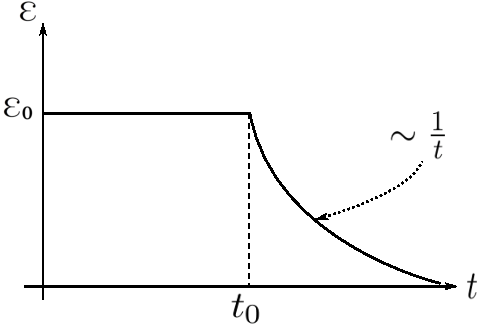
\includegraphics[height=5cm]{section4_fig4} 
  \caption{Annealing schedule ($t$ is the number of iterations)}
  \label{fig:annealingScheduleKMeans}
\end{figure}



% -----------------------------------------------------------------------------

\subsubsection{Number of Prototypes}
The number of prototypes is a hyperparameter of k-means clustering. Knowledge about the data (noise amplitude) and robustness of the clustering solution can guide this choice. 

\paragraph{choice of resolution}
\[ \begin{array}{ll}
	\includegraphics[width=6cm]{section4_fig5}
	& \begin{array}{l}
		\text{1 cluster} \\
		\text{3 cluster} \\
		\text{9 cluster} \\
		\text{many cluster?} \\\\
		\Rightarrow \substack{	\text{additional prior} \\
					\text{knowledge is needed!}}
	\end{array}
\end{array} \]
$E_{\min}^T$: average size of cluster (in terms of variance)
\begin{itemize}
	\itl large for few clusters -- small for many clusters
	\itl zero, if number of cluster $\corresponds$ number of data points
\end{itemize}
Note that $E^T_\mathrm{min}$ goes down if $M$ increases.
\\

The choice of resolution should depend prior knowledge on the average
size of the cluster (e.g.\ clusters ``smaller'' than the variance of noise probably do not capture meaningful structure). 
\begin{itemize}
	\itr exploit prior knowledge on $E_{\min}^T$ 
        (e.g.\ $E_{\min}^T \geq \sigma_\mathrm{noise}^2$ which is a natural boundary on 
        $E^T_\mathrm{min}$ )
\end{itemize}
This prior knowledge can be exploited using the heuristic of
\emph{iterative refinement}, as illustrated in algorithm \ref{alg:iterative-k-means-refinement}.

\begin{algorithm}
\DontPrintSemicolon
initialization: $\vec{w}_1 = \frac{1}{p} \sum\limits_{\alpha} 
	\vec{x}^{(\alpha)}, \underbrace{ \big( E_{\min}^T \big)^* }_{
			\substack{	\text{desired minimal} \\
					\text{average variance}} }
		, M = 1$ \;
\Begin(loop){
\lIf{$E_{\min}^T < \big( E_{\min}^T \big)^*$}{STOP} \;
select partition $q \in \{ 1, \ldots, M \}$ with largest variance
\[ q = \argmax_{\gamma} \left( \frac{\sum\limits_{\alpha} m_\gamma^{(\alpha)}
  \big( \vec{x}^{(\alpha)} - \vec{w}_\gamma \big)^2}{\sum\limits_{\alpha}
  m_\gamma^{(\alpha)}} \right) \]
add a new prototype:  $\vec{w}_{M+1} = \vec{w}_q + 
\underbrace{ \vec{\eta}_q }_{ \substack{	\text{small random} \\
    \text{vector}} }$\;
$M \leftarrow M + 1$\\
do k-means clustering with these $M$ prototypes \\
}
\label{alg:iterative-k-means-refinement}
\caption{iterative k-means refinement}
\end{algorithm}

\paragraph{Robustness of clustering solution}\mbox{}\\\\
\emph{Idea:} If the solution captures meaningful structure in the
data, multiple runs of the same algorithm with different initial
conditions should yield similar solutions.
\\\\
\emph{Caveat:} Assignment of labels to clusters is arbitrary: permutation of labels does
neither change cost nor character of the solution. 
\[ \begin{array}{l}
	1, 2, 3, \ldots, M \\
	9, 1, M, \ldots, 7
      \end{array} 
\]
This ``permutation symmetry''leads to $M!$ trivially equivalent optima, so the robustness-criterion needs to account for such equivalence classes of optima.  
The number of equivalence class increases with increasing number of prototypes
$\leadsto$ structurally different equivalent classes to be compared!


How many prototypes? $\rightarrow$ increase number until
''overfitting'' occurs
\begin{itemize}
  \itl many equivalence classes with approximately equal cost
  \itl different initial conditions and different sequences of pattern 
  presentation lead to clustering solutions from different 
  equivalence classes
  \itl different sub-datasets lead to solutions from different 
  equivalence classes
\end{itemize} 

\paragraph{Validation measure}\mbox{}\\\\
\textcite{LangeEtAl2004} estimate expected dissimilarity between
solutions for different samples from the same dataset $\leadsto$
``best'' number of clusters yields most robust clustering (highest
similiarity). For further details, see \textcite{Luxburg2010}. 
\begin{itemize}
\item Model free approaches:  Stability based validation
\item \textbf{Idea:} taking to many or too few clusters leads to unstable partitions
\item $\mathbf{X} = \big\{ \vec{x}^{(\alpha)} \big\}, \alpha = 1, \ldots, p; \quad \vec{x} \in \mathbb{R}^N$ ;\
A solution of the clustering algorithm is $\mathbf{Y} =(y_{1}, \ldots , y_{p})$ where $y_{i} \in L:=\{1,\ldots,M\}$
\item Comparing clustering solutions $Y_{1}$ and $Y_{2}$:\\
$$d:= \frac{1}{|\mathbf{Y_1}|}
      \sum_\alpha \mathbf{1}\left\{Y_{1, \alpha}\neq Y_{2, \alpha} \right\}\qquad$$ 
\end{itemize}
\begin{algorithm}
\DontPrintSemicolon
\Begin (for each $M \in \{M_{min},\ldots,M_{max} \}$){
\Begin(loop for $r$ splits of data){
Split data $\mathbf{X}$ into $\mathbf{X}_1^{(i)}$ and $\mathbf{X}_2^{(i)}$ and find corresponding clustering solutions $\mathbf{Y}_{1}^{(i)}$ and $\mathbf{Y}_{2}^{(i)}$  \\
Compute dissimilarity $d_i:= \frac{1}{|\mathbf{X}_2|}
      \sum_\alpha \mathbf{1}\left\{\mathbf{Y_2}^{(\alpha)}\neq \phi_1[\mathbf{X}_2^{(\alpha)}]\right\}\qquad $\\
      Where $\phi_1$ denotes the label of the nearest prototype taking into account permutations\\
       
}
Compute average dissimilarity: $\hat{S}_{clustering}= \frac{1}{r}\sum_r d_i$ \\~\\
Sample $s$ random clustering assignments and compute estimate average of the distances to estimate  $\hat{S}_{random}$ \\~\\
Calculate stability index:  $\bar{S}_M = \frac{\hat{S}_{clustering}}{\hat{S}_{random}}$ \\
}
Return $\hat{M} = \argmin_M(\bar{S}_M)$

\caption{Validation measure}
\end{algorithm}
\slideref{slide: K-means Gaussian data}
\paragraph{Alternative clustering approaches}\mbox{}\\
\begin{itemize}
 \item  density based models (``model-based'' $\Rightarrow$ Gaussian Mixture algorithm)
 \item  hierarchical (connectivity based) clustering 
 \begin{itemize}
 \item single linkage ($\sim$ nearest neighbor)
 \item complete linkage
 \item average linkage / within group ssq (Ward criterion)
 \item agglomerative vs.\ divisive clustering
\end{itemize}
\end{itemize}

% -----------------------------------------------------------------------------
\subsection{Pairwise Clustering Methods}
% -----------------------------------------------------------------------------
In some applications, direct measurements of the objects to be
clustered are not available. If information regarding object
similarities or distances between objects is available, clustering
($\sim$ grouping objects that are similar to each other) is still
possible. In this setting, too, mean field approaches provide
effective means to find good clustering solutions
\citep{HofmannBuhmann1997}.


\subsubsection{The Clustering Problem}
\emph{observations:} set of $p$ ''objects'' $\alpha, \alpha = 1, \ldots, p$ 
\\\\
\emph{distance matrix} $\big\{ d_{\alpha \alpha^{'}} \big\}$
\[ \begin{array}{ll}
	\begin{array}{c|ccccc}
	& 1 & 2 & 3 && p \\
	\hline \\
	1 & 0 & 1.7 & 0.99 && 3.0 \\
	2 & 1.7 & 0 & 0.3 & \ldots & 0.1 \\
	3 & 0.9 & 0.3 & 0 && 0.2 \\
	\vdots && \vdots && \ddots & \vdots \\
	p & 3.0 & 0.1 & 0.2 & \ldots & 0
	\end{array}
	& \substack{	\text{relational representation} \\
			\text{''pairwise data''}}
\end{array} \]
Commonly chosen constraints on the distance matrix e.g.\ are zero-diagonal, symmetry, or distances fulfilling the triangle-inequality. Examples are:  
\begin{itemize}
\item distances directly determined by measurements
  (e.g. dissimilarity judgements in a psychophysics experiment, e.g.\
  confusion matrices)
\item distances determined through algorithms (e.g. dissimilarity of
  protein sequences through sequence alignment procedures,
  graph-similarity measures) 
\item distances derived from an underlying vector space representation
  \begin{equation}
    \Big( d: \mathbb{R}^N \text{ x } \mathbb{R}^N 
    \rightarrow \mathbb{R}_0^+, \text{ e.g. }
    d_{\alpha \alpha^{'}} = \frac{1}{2} \big(
    \vec{x}^{(\alpha)} - \vec{x}^{(\alpha^{'})} \big)^2
    \Big)
  \end{equation}
\item elements derived via a ''kernel trick'' ({\it cf. chapter
    2.3.3})
		\begin{equation}
                  \vec{\phi}: \vec{x}^{(\alpha)} \rightarrow
                  \vec{\phi}_{\big( \vec{x}^{(\alpha)} \big)}
                  \equiv \vec{\phi}^{(\alpha)}
		\end{equation}
		\begin{equation}
			\begin{array}{ll}
			d_{\alpha \alpha^{'}} 
			& = \frac{1}{2} \big( \vec{\phi}^{(\alpha)} 
				- \vec{\phi}^{(\alpha^{'})} \big)^2 \\\\
			& = \frac{1}{2} \Big\{ \big( \vec{\phi}^{(\alpha)}
				\big)^2 - 2\big( \vec{\phi}^{(\alpha)} \big)^T
				\vec{\phi}^{(\alpha^{'})} + \big(
				\vec{\phi}^{(\alpha^{'})} \big)^2 \Big\} \\\\
			& = \frac{1}{2} \bigg\{ k_{\big( \vec{x}^{(\alpha)},
				\vec{x}^{(\alpha)} \big)} 
				+ k_{\big(\vec{x}^{(\alpha^{'})},
				\vec{x}^{(\alpha^{'})} \big)}
				- 2k_{\big(\vec{x}^{(\alpha)},
				\vec{x}^{(\alpha^{'})} \big)}
				\bigg\}
			\end{array}
                      \end{equation}
\end{itemize}
{\bf cluster models}
\\\\
set of clusters (partitions): $q = 1, \ldots, M$
\\\\
binary assignment variables:
\begin{equation}
	m_q^{(\alpha)} \left\{ \begin{array}{ll}
		1, & \text{if object } \alpha \text{ belongs to cluster } q \\\\
		0, & \text{else}
	\end{array} \right. 
\end{equation}
cost function:
\begin{equation}
	E_{ \big[ \big\{ m_q^{(\alpha)} \big\} \big] }
	= \frac{1}{2p} \sum\limits_q^M \sum\limits_{\alpha}
	m_q^{(\alpha)} \underbrace{ \frac{\sum\limits_{\alpha^{'}} 
		m_q^{(\alpha^{'})} d_{\alpha \alpha^{'}}}{
                \sum\limits_{\alpha'} m_q^{(\alpha')}
		}}_{ \substack{	\text{av. distance between} \\
				\alpha \text{ and other objects $\alpha'$} \\
				\text{from the same cluster } q}}
	= \frac{1}{2p} \sum\limits_q 
	 \frac{\sum\limits_{\alpha \alpha^{'}} m_q^{(\alpha)}
		m_q^{(\alpha^{'})} d_{\alpha \alpha^{'}}}{
			\sum\limits_{\alpha} m_q^{(\alpha)} }
\end{equation}
where $\sum\limits_{\alpha} m_q^{(\alpha)}$ is simply the number of objects assigned to cluster $q$.\\\\ 
model selection:
\begin{equation}
	E \eqexcl \min
\end{equation}

% -----------------------------------------------------------------------------
\subsubsection{Pairwise Clustering with Euclidean Distances}
\label{sec:pairwiseEuclidean}
observations (feature vectors): $\vec{x}^{(\alpha)}, \alpha = 1, \ldots, p; \vec{x}^{(\alpha)} = \mathbb{R}^N$ 
\\\\
distance measure:
\begin{equation}
	d_{\alpha \alpha^{'}} = \frac{1}{2} \big( \vec{x}^{(\alpha)} 
		- \vec{x}^{(\alpha^{'})} \big)^2
\end{equation}
\begin{equation}
	\begin{array}{ll}
	E_{\big[ \big\{ m_q^{(\alpha)} \big\} \big]}
	& = \frac{1}{2p} \sum\limits_q \frac{ \sum\limits_{\alpha \alpha^{'}}
		m_q^{(\alpha)} m_q^{(\alpha^{'})} \big( \vec{x}^{(\alpha)}
		-\vec{x}^{(\alpha^{'})} \big)^2 }{
			\sum\limits_{\alpha} m_q^{(\alpha)}} \\\\
	& = \frac{1}{2p} \sum\limits_q \frac{ \sum\limits_{\alpha \alpha^{'}}
		m_q^{(\alpha)} m_q^{(\alpha^{'})} \Big\{ \big( 
		\vec{x}^{(\alpha)} \big)^2 - 2\big( \vec{x}^{(\alpha)} \big)^T
		\vec{x}^{(\alpha^{'})} + \big( \vec{x}^{(\alpha^{'})} \big)^2
		\Big\} }{ \sum\limits_{\alpha} m_q^{(\alpha)} } \\\\
	& = \frac{1}{2p} \sum\limits_q \Bigg\{ \sum\limits_{\alpha}
		m_q^{(\alpha)} \big( \vec{x}^{(\alpha)} \big)^2 
		- 2 \Big( \sum\limits_{\alpha} m_q^{(\alpha)} \big( 
		\vec{x}^{(\alpha)} \big)^T \Big) 
		\underbrace{ \frac{ \sum\limits_{\alpha^{'}} m_q^{(\alpha^{'})} 
		\vec{x}^{(\alpha^{'})} }{ \sum\limits_{\alpha^{'}} 
		m_q^{(\alpha^{'})} } }_{
			\substack{ \eqexcl \vec{w}_q \\
				\substack{\text{centroid =} \\ 
                                  \text{center of mass}\\ \text{ ({\it cf. \ref{kmeans_modelselection}})}}} }
		+ \sum\limits_{\alpha} m_q^{(\alpha)} \big( \vec{x}^{(\alpha)}
			\big)^2 \Bigg\} \\\\
	& = \frac{1}{p} \sum\limits_{q, \alpha} m_q^{(\alpha)} \Big\{
		\big( \vec{x}^{(\alpha)} \big)^2 - \big( \vec{x}^{(\alpha)}
		\big)^T \vec{w}_q \Big\} \\\\
	& = \frac{1}{p} \sum\limits_{q, \alpha} m_q^{(\alpha)} \Big\{
		\big( \vec{x}^{(\alpha)} \Big)^2 - \big( \vec{x}^{(\alpha)}
		\big)^T \vec{w}_q - \underbrace{ \vec{w}_q^2 }_{
			= \frac{ \sum\limits_{\alpha} m_q^{(\alpha)} \big(
				\vec{x}^{(\alpha)} \big)^T }{
					\sum\limits_{\alpha} m_q^{(\alpha)}}
			\cdot \vec{w}_q}
		+ \vec{w}_q^2 \Big\} \\\\
	& = \frac{1}{p} \sum\limits_{q, \alpha} m_q^{(\alpha)} \Big\{ 
		\big( \vec{x}^{(\alpha)} \big)^2 - 2 \big( \vec{x}^{(\alpha)}
		\big)^T \vec{w}_q + \vec{w}_q^2 \Big\} \\\\
	& = \frac{1}{p} \sum\limits_{q, \alpha} m_q^{(\alpha)} \big( 
		\vec{x}^{(\alpha)} - \vec{w}_q \big)^2 \\\\
	& = E_{\big[ \big\{ m_q^{(\alpha)} \big\}, \big\{ \vec{w}_q \big\} \big]} 
 \corresponds \text{ cost function eq.(\ref{eq:euclideanClusterCost})}
	\end{array}
\end{equation}
K-means Clustering $\corresponds$ Pairwise Clustering with squared Euclidean distance

% -----------------------------------------------------------------------------

\subsubsection{The Mean-Field Approximation for Pairwise Clustering}
discrete (binary) optimization problem:
\begin{equation}
	E_{ \big[ \big\{ m_q^{(\alpha)} \big\} \big] }
	= \frac{1}{2p} \sum\limits_q \frac{\sum\limits_{\alpha \alpha^{'}}
		m_q^{(\alpha)} m_q^{(\alpha^{'})} d_{\alpha \alpha^{'}}}{
			\sum\limits_{\alpha^{'}} m_q^{(\alpha^{'}}}
	\eqexcl \min
\end{equation}
\begin{itemize}
	\itR gradient-based methods are not applicable
	\itR methods from combinatorial optimization are needed
\end{itemize}

\[ \begin{array}{ccc}
  \text{simulated annealing}
  & \text{vs.}
  & \text{mean-field annealing} \\
  \text{\scriptsize straightforward but slow}
  && \substack{ 	\text{approximation} \\
    \text{why? good and fast!}}
\end{array} 
\]
We can apply the framework of section \ref{sec:mean-field-annealing}
but:
\begin{itemize}
	\itl variables $m_q^{(\alpha)}$ are \emph{normalized} to $\sum\limits_q
		m_q^{(\alpha)} = 1$ 
	\itl calculation of moments and mean-fields must be adapted because marginalized variables are not independent anymore
\end{itemize}
\textbf{Nomenclature:} Using the \emph{set-product} $\otimes$ we define\\\\
\begin{tabular}{r l p{9cm}}
$\big\{ \vec{m}^{(\alpha)} \big\}$: & & set of all $M$-dimensional binary vectors $\big( m_1^{(\alpha)}, m_2^{(\alpha)}, \ldots, 
  m_M^{(\alpha)} \big)^T$ which fulfill the normalization condition: exactly one element equals 1. \\\\
$\mathscr{M}$: & & $\big\{ \vec{m}^{(1)} \big\} \otimes \big\{ \vec{m}^{(2)} \big\} \otimes \ldots \otimes \big\{ \vec{m}^{(p)} \big\}$\\
& & Kartesian product between all possible binary assignment variables i.e.\ all possible valid assignments for the full dataset\\\\
$\mathscr{M}_{\gamma}$:& &  $\big\{ \vec{m}^{(1)} \big\} \otimes \ldots \otimes \big\{ \vec{m}^{(\gamma - 1)} \big\} \otimes
  \big\{ \vec{m}^{(\gamma + 1)} \big\} \otimes \ldots \otimes
  \big\{ \vec{m}^{(p)} \big\}$\\
& & i.e.\ set of all possible assignments for all datapoints except $\gamma$
\end{tabular}
\\\\
assignment noise $\rightarrow$ Gibbs distribution
\begin{equation}
	P_{ \big( \big\{ m_q^{(\alpha)} \big\} \big) }
	= \frac{1}{Z_p} \exp \Big\{ -\beta 
		E_{\big[ \big\{ m_q^{(\alpha)} \big\} \big]}^p
		\Big\}
\end{equation}
where
\begin{equation}
	Z_p = \sum\limits_{\mathscr{M}} \exp \Big\{ -\beta
		E_{\big[ \big\{ m_q^{(\alpha)} \big\} \big]}^p
		\Big\}
\end{equation}
factorizing distribution
\begin{equation}
	Q_{ \big[ \big\{ m_q^{(\alpha)} \big\} \big] }
	= \frac{1}{Z_Q} \exp \Big\{ -\beta \sum\limits_{p, \gamma}
		m_p^{(\gamma)} \underbrace{ e_p^{(\gamma)} }_{
			\text{{\tiny mean-fields}} } \Big\}
\end{equation}
where:
\begin{equation}
	Z_Q = \sum\limits_{\mathscr{M}} \exp \Big\{ -\beta \sum\limits_{p, 
		\gamma} m_p^{(\gamma)} e_p^{(\gamma)} \Big\}
\end{equation}
this allows to calculate the \emph{first moments} w.r.t $Q$ ($\rightarrow$
assignment probabilities).
\begin{equation}
	\big< m_q^{(\gamma)} \big>_Q
	= \frac{1}{Z_Q} \sum\limits_{\mathscr{M}} m_q^{(\gamma)}
		\exp \Big\{ -\beta \sum\limits_{r, \delta} 
		m_{r}^{(\delta)} e_{r}^{(\delta)} \Big\}
\end{equation}
using the factorization eq.~(\ref{eq:factorizingMoments}) regarding valid assignments $\big\{ \vec{m}^{(\gamma)} \big\}$ for observation $\gamma$ and the rest of the variables  this simplifies (for any functions $f,g$) to:
\begin{equation}
	\sum\limits_{\mathscr{M}} \bigg[ f_{ \big( \big\{ m_p^{(\delta)} 
		\big| \delta \neq \gamma \big\} \big) }
		\cdot g_{ \big\{ m_p^{(\delta)} \big| \delta = \gamma 
			\big\} \big) }
		\bigg]
	= \bigg[ \sum\limits_{\mathscr{M}_{\gamma}} f_{ \big( \big\{ 
		m_p^{(\delta)} \big| \delta \neq \gamma \big\} \big) }
		\bigg] \cdot \bigg[ \sum\limits_{\big\{ \vec{m}^{(\gamma)} 
			\big\} } g_{ \big\{ m_p^{(\delta)} \big| \delta = 
			\gamma \big\} \big) } \bigg]
\end{equation}
and finally gives
%% this formula has been seriously confusing / wrong (indices?) so double check
\begin{equation}
	\begin{array}{ll}
	\big< m_q^{(\gamma)} \big>_Q
	& = \frac{ \Bigg[ \sum\limits_{\mathscr{M}_{\gamma}} \exp \Big\{ -\beta
		\sum\limits_{r, \delta \neq \gamma} m_{r}^{(\delta)}
		e_{r}^{(\delta)} \Big\} \Bigg] \cdot \Bigg[ 
		\overbrace{ \sum\limits_{ \big\{ \vec{m}^{(\gamma)} \big\} }
		m_q^{(\gamma)} }^{\substack{	\text{only term with} \\
						m_q^{(\gamma)} = 1 \\
						\text{remains} }}
		\exp \Big\{ -\beta \sum\limits_{r} m_{r}^{(\gamma)}
		e_{r}^{(\gamma)} \Bigg] }{
			\underbrace{
			\Bigg[ \sum\limits_{\mathscr{M}_{\gamma}} \exp 
			\Big\{ -\beta \sum\limits_{r, \delta \neq \gamma} 
			m_{r}^{(\delta)}e_{r}^{(\delta)} \Big\} \Bigg]
			}_{ \text{first terms cancel} } 
			\cdot \Bigg[ \sum\limits_{ \big\{ \vec{m}^{(\gamma)} 
			\big\} } \exp \Big\{ -\beta
			\underbrace{ \sum\limits_{r} m_{r}^{(\gamma)}
				e_{r}^{(\gamma)} }_{
				\substack{	\text{only one term of this} \\
						\text{sum remains for every} \\
						\text{term of the qrevious }
						\text{sum}} }
				\Big\} \Bigg] } \\\\
	 & = \frac{ \exp \big\{ -\beta\, m_q^{(\gamma)} e_q^{(\gamma)} \big\} }{
	 	\sum\limits_{r} \exp \big\{ -\beta \,
	 	m_{r}^{(\gamma)} e_{r}^{(\gamma)} \big\} }
	\; \underbrace{=}_{\substack{\text{only the } \\ m_r^{(\gamma)} = 1 \\\text{ stays}}} \; \underbrace{\frac{ \exp \big\{ -\beta e_q^{(\gamma)} \big\} }{
		\sum\limits_{r} \exp \big\{ -\beta 
		e_{r}^{(\gamma)} \big\} }}_{\text{soft-max of the mean-fields}}
	\end{array}
\end{equation}
% before replacing q->r, p->q
% \begin{equation}
%         \begin{array}{ll}
%         \big< m_p^{(\gamma)} \big>_Q
%         & = \frac{ \Bigg[ \sum\limits_{\mathscr{M}_{\gamma}} \exp \Big\{ -\beta
%                 \sum\limits_{q, \delta \neq \gamma} m_{q}^{(\delta)}
%                 e_{q}^{(\delta)} \Big\} \Bigg] \cdot \Bigg[ 
%                 \overbrace{ \sum\limits_{ \big\{ \vec{m}^{(\gamma)} \big\} }
%                 m_p^{(\gamma)} }^{\substack{    \text{only term with} \\
%                                                 m_p^{(\gamma)} = 1 \\
%                                                 \text{remains} }}
%                 \exp \Big\{ -\beta \sum\limits_{q} m_{q}^{(\gamma)}
%                 e_{q}^{(\gamma)} \Bigg] }{
%                         \underbrace{
%                         \Bigg[ \sum\limits_{\mathscr{M}_{\gamma}} \exp 
%                         \Big\{ -\beta \sum\limits_{q, \delta \neq \gamma} 
%                         m_{q}^{(\delta)}e_{q}^{(\delta)} \Big\} \Bigg]
%                         }_{ \text{first terms cancel} } 
%                         \cdot \Bigg[ \sum\limits_{ \big\{ \vec{m}^{(\gamma)} 
%                         \big\} } \exp \Big\{ -\beta
%                         \underbrace{ \sum\limits_{q} m_{q}^{(\gamma)}
%                                 e_{q}^{(\gamma)} }_{
%                                 \substack{      \text{only one term of this} \\
%                                                 \text{sum remains for every} \\
%                                                 \text{term of the previous }
%                                                 \text{sum}} }
%                                 \Big\} \Bigg] } \\\\
%          & = \frac{ \exp \big\{ -\beta\, m_p^{(\gamma)} e_p^{(\gamma)} \big\} }{
%                 \sum\limits_{q} \exp \big\{ -\beta \,
%                 m_{q}^{(\gamma)} e_{q}^{(\gamma)} \big\} }
%         \; \underbrace{=}_{\substack{\text{only the } \\ m_q^{(\gamma)} = 1 \\\text{ stays}}} \; \underbrace{\frac{ \exp \big\{ -\beta e_p^{(\gamma)} \big\} }{
%                 \sum\limits_{q} \exp \big\{ -\beta 
%                 e_{q}^{(\gamma)} \big\} }}_{\text{soft-max of the mean-fields}}
%         \end{array}
% \end{equation}
The $\big< m_q^{(\gamma)} \big>_Q \in [0, 1]$ represent assignment
probabilities, i.e.\ they quantify the probability that an object
belongs to a cluster (since we have $\sum_r \langle m_r^{(\gamma)} \rangle = 1$).
\begin{itemize}
	\itl $\beta \rightarrow \infty: \big< m_q^{(\gamma)} \big>_Q
		\rightarrow \{0, 1\}$ ''hard assignments'' (cmp.\ k-means)
\end{itemize}
minimization of the KL-divergence (eq. \ref{eq:MeanfieldEquation}) leads to:
\begin{equation}
	\frac{\partial \big< E^p \big>_Q}{\partial e_q^{(\alpha)}}
	- \sum\limits_{r, \gamma} \frac{
		\overbrace{ \partial \big< m_r^{(\gamma)} \big>_Q }^{
			\substack{	\text{depends only on} \\
					\text{data point } \gamma (\text{ not } \alpha)}}}{
			\partial e_q^{(\alpha)}}
		e_r^{(\gamma)} \eqexcl 0
\end{equation}
\begin{equation}
	\frac{\partial \big< E^p \big>_Q}{\partial e_q^{(\alpha)}}
	- \sum\limits_r \frac{\partial \big< m_r^{(\alpha)} \big>_Q}{
		\partial e_q^{(\alpha)}}
		e_r^{(\alpha)} \eqexcl 0
\end{equation}
for the mean-fields we obtain
\begin{equation}
	\begin{array}{lll}
	e_q^{(\alpha)}
	& = & \frac{1}{p} \Bigg[ \frac{\sum_{\alpha',\gamma}}{\sum\limits_{\gamma} \big<
		m_q^{(\gamma)} \big>_Q} \bigg\{ d_{\alpha \alpha^{'}}
		-\frac{1}{\sum\limits_{\gamma} \big< m_q^{(\gamma)} \big>_Q}
		\sum\limits_{\delta \neq \alpha} \big< m_q^{(\gamma)} \big>_Q
		d_{\delta\delta} \bigg\} \\\\
	&& + \frac{1}{\sum\limits_{\gamma}
		\big< m_q^{(\gamma)} \big>_Q } \sum\limits_{\delta \neq \alpha}
		\big< m_q^{(\delta)} \big>_Q \bigg\{ \big( d_{\delta \alpha}
		+ d_{\alpha \delta} \big) - \frac{1}{2} \frac{1}{
		\sum\limits_{\gamma} \big< m_q^{(\gamma)} \big>_Q} \\\\
	&& \sum\limits_{\varepsilon \neq \delta, \alpha} 
		\big< m_q^{(\varepsilon)} \big>_Q \cdot \big( d_{\delta 
		\varepsilon} + d_{\varepsilon \delta} \big) \bigg\} \Bigg]
	\end{array}
\end{equation}
{\it proof: supplementary material}
\\\\
The terms $ d_{\delta \alpha} + d_{\alpha \delta}$ and $d_{\delta
  \varepsilon} + d_{\varepsilon \delta}$ illustrate that the
mean-field approximation leads to an evaluation of the symmetrized
distance matrix. 
\\\\
Therefore, a common assumption wrt.\ the \emph{distance matrix} is:
\begin{itemize}
	\itl symmetric: $d_{\alpha,\alpha'}=d_{\alpha',\alpha}$
	\itl diagonal elements $d_{\alpha \alpha^{'}} \eqexcl 0$
\end{itemize}
Under this assumption, the mean-fields simplify as:
\begin{equation}\label{eq:simplifiedMeanFields}
	e_q^{(\alpha)} = \underbrace{
	\frac{2}{p} \frac{1}{\sum\limits_{\gamma} \big< m_q^{(\gamma)} \big>_Q}
	\sum\limits_{\delta} \big< m_q^{(\delta)} \big>_Q 
	\underbrace{ \Bigg\{ d_{\delta \alpha} - \frac{1}{2} \frac{1}{
		\sum\limits_{\gamma} \big< m_q^{(\gamma)} \big>_Q} 
		\sum\limits_{\varepsilon} \big< m_q^{(\varepsilon)} \big>_Q
		d_{\varepsilon \delta} \Bigg\} }_{
		\substack{	\text{distance between data objects } \alpha
				\text{ and } \delta, \\
				\text{corrected by the average distance between}
				\\
				\text{objects of the cluster, to which } \delta
				\text{ belongs (here: } q \text{) } }}
	}_{ \substack{	\text{average corrected distance between data objects}\\
			\alpha \text{ and all objects } \delta \text{ of cluster } q}}
\end{equation}
interpretation of the ``mean fields'':
\begin{itemize}
  \itR ''metric visualization'' of the $e_q^{(\alpha)}$:
  \begin{center}
    \includegraphics[width=6cm]{section4_fig6}
  \end{center}
  \itR mean-fields depend on assignment probabilities $\big<
  m_q^{(\alpha)} \big>_Q$ rather than on the ''hard'' binary
  assignments
  \begin{itemize}
    \itl this is an effect of the underlying stochastic optimization
    procedure \itl ''fuzzy'' memberships: objects contribute only
    weighted by their probability $\big< m_q^{(\alpha)} \big>_Q$ of
    assignment
  \end{itemize}
  \itR assignment probabilities $\big< m_1^{(\alpha)} \big>_Q$ depend
  on the average normalized distance between the object $\alpha$ under
  consideration and the objects of cluster $q$ (probability is high,
  if distance to $\alpha$ is small compared to average distance within
  cluster).  
\end{itemize}

\paragraph{Euclidean distances:} As shown above, using Euclidean distance as a pairwise similarity measure is a special case and yields particularly simple expressions for the mean fields and prototypes.
\\\\
For observations (feature vectors): $\vec{x}^{(\alpha)}; \alpha = 1,
\ldots, p; \vec{x}^{(\alpha)} \in \mathbb{R}^N$ and euclidean distance
measure:
\begin{equation}
	d_{\alpha \alpha^{'}} 
	= \frac{1}{2} \big( \vec{x}^{(\alpha)} - \vec{x}^{(\alpha^{'})}
		\big)^2
\end{equation}
we then obtain:
\begin{equation}
	e_q^{(\alpha)} 
	= \frac{1}{2} \big( \vec{x}^{(\alpha)} - \vec{w}_q \big)^2
\end{equation}
with
\begin{equation}
	\vec{w}_q 
	= \underbrace{ \frac{\sum\limits_{\gamma} \big< m_q^{(\gamma)} \big>_Q 
		\vec{x}^{(\gamma)}}{\sum\limits_{\gamma}
		\big< m_q^{(\gamma)} \big>_Q} }_{
		\substack{	\text{center of mass of all objects weighted} \\
				\text{by their probability of assignment}} }
\end{equation}
{\it proof: supplementary material}
\begin{itemize}
      \itl probabilistic cluster assignments. thus:
	\itl natural extension of K-means clustering to the case of ''fuzzy''
		assignments
\end{itemize}

% -----------------------------------------------------------------------------

\subsubsection{General Mean-Field Algorithm for Pairwise Clustering}
\label{sec:generalPairwiseClustering}
Algorithm \ref{alg:meanFieldClustering} implements the stochastic
optimization procedure (mean field annealing) from chapter
\ref{sec:mean-field-annealing} to find nearly optimal cluster centers
and assignment (probabilities) of data points to these clusters.
\begin{algorithm}
  \DontPrintSemicolon
  \textbf{Initialization:}\;
  - choose number $M$ of partitions (max no)\;
  - choose initial  ($\beta_0$) and final  ($\beta_f$) values of the noise parameter\;
  - choose annealing factor  $\eta$ and convergence criterion  $\theta$\;
  - initialize mean-fields  $e_q^{(\alpha)}$ with random numbers $\in [0, 1]$\;

- set $\beta \leftarrow \beta_0$\;
\While(annealing){$\beta < \beta_f$}{
\Repeat(EM fixpoint iteration){
$\big| \big( e_q^{(\alpha)} \big)_{\mathrm{new}}
	- \big( e_q^{(\alpha)} \big)_{\mathrm{old}} \big| < \theta 
	\text{ for all }q, \alpha$}{
compute assignment probabilities\;
\[ \big< m_q^{(\alpha)} \big>_Q = \frac{ \exp \big\{ -\beta \big(e_q^{(\alpha)}
	\big)_{\mathrm{old}}\big\} }{ \sum\limits_r \exp \big\{ -\beta \big(
	e_r^{(\alpha)} \big)_{\mathrm{old}} \big\} } \text{ for all }
	q, \alpha
\]
compute new mean-fields\;
\[ \begin{array}{lll}
   \big( e_q^{(\alpha)} \big)_{\mathrm{new}} 
   	& = & \frac{2}{M} \frac{1}{
	\sum\limits_{\gamma} \big< m_q^{(\gamma)} \big>_Q } \sum\limits_{\delta}
	\big<m_q^{(\delta)} \big>_Q \\\\
	&& \cdot \bigg\{ d_{\delta \alpha} - \frac{1}{2} \frac{1}{
		\sum\limits_{\gamma} \big< m_q^{(\gamma)} \big>_Q }
		\sum\limits_{\varepsilon} \big< m_q^{(\varepsilon)}
		\big>_Q d_{\varepsilon \delta} \bigg\}
	\text{ for all } q, \alpha
   \end{array}
\]
}
$\beta \leftarrow \eta \cdot \beta$\;
}
\label{alg:meanFieldClustering}
\caption{soft k-means clustering for general distances}
\end{algorithm}

\paragraph{Application example:} \label{sec:application-example}
clustering of protein sequences
\\\\
definition of a distance measure:
\begin{itemize}
	\itl pairwise sequence alignment 
	\itl definition of distance on the basis of number of insertions, 
		deletions and amino acid exchanges ('edit' distance)
\end{itemize}
\slideref{slide: Clustering of protein sequences}
In a similar way, spiketrains can be clustered to identify groups of cells with similar response properties ($\leadsto$ spiketrain metrics).\\ 


% -----------------------------------------------------------------------------

\subsubsection{Missing Data}
The algorithm for pairwise data lends itself in a natural way do deal with \emph{missing data} or subsets of data to reduce computational burden (e.g\ when computing distances is costly). 
\begin{itemize}
	\itl number of matrix elements $\sim p^2$ 
	\itl calculation or measurement of all distances may be computationally
		expensive or even unfeasible
	\itl distance matrices are often ''redundant'' $\leadsto$ not all
		matrix entries might be needed (e.g., position on plane: 3 dists. enough)
\end{itemize}
As can be seen from the average distance of data object $\alpha$ to
all data objects of cluster $q$:
\begin{equation}
	\overline{d}_{q \alpha} 
	= \frac{\sum\limits_{\gamma} \big< m_q^{(\gamma)} \big>_Q 
		d_{\gamma \alpha} }{ \sum\limits_{\gamma} \big<
		m_q^{(\gamma)} \big>_Q}
\end{equation}
and the mean fields (see eq.~\ref{eq:simplifiedMeanFields}) can be written in termns of these:
\begin{equation}
	e_q^{(\alpha)} 
	= \bigg\{ \overline{d}_{q \alpha} - \frac{1}{2} \sum\limits_{\delta}
		\big< m_q^{(\delta)} \big>_Q \overline{d}_{q \delta} \bigg\}
		\cdot \frac{2}{M}
\end{equation}
These computations depend only on the \emph{average} distances and therefore enable the following \emph{missing data heuristics}:
\begin{itemize}
	\itR estimate average values $\overline{d}_{p \alpha}$ using the 
		measured distances only
	\itR perform summations within $\overline{d}_{p \alpha}$ only over the
		available distances
\end{itemize}
Good choice of a subset of data to compute the average values can
significantly speed up clustering without strongly changing the solution.

% -----------------------------------------------------------------------------



\subsubsection[Euclidean soft k-means clustering]{Special case: ''soft'' K-means with Euclidean distances}
Using the \emph{squared euclidean distance} as the distance measure in
the general procedure of algorithm \ref{alg:meanFieldClustering}
yields a particularly simple version of the soft clustering procedure
that is described in algorithm \ref{alg:softKmeansEuclidean}. It is robust, fast, and allows to choose $k$. 

\begin{algorithm}
  \DontPrintSemicolon
  \textbf{Initialization:}\;
 - choose no. $M$ of partitions (max no)\; 
- choose initial ($\beta_0$) and final ($\beta_f$) values of the noise parameter\;
- initialize prototypes:  $\vec{w}_q = \frac{1}{p} 
\sum\limits_{\alpha} \vec{x}^{(\alpha)} + \vec{\eta}_q$ (small random vector)\;
- choose annealing factor $\eta$\;
- choose convergence criterion $\theta$\;
- $\beta \leftarrow \beta_0$\;
  \While{$\beta < \beta_f$ (annealing)}{
\Repeat( EM){$\big| \vec{w}_q^{\mathrm{new}} - \vec{w}_q^{\mathrm{old}} \big| < \theta$ for all $q$}{
compute assignment probabilities
\[ \big< m_q^{(\alpha)} \big>_Q = \frac{ \exp \big\{ -\frac{\beta}{2}
	\big( \vec{x}^{(\alpha)} - \vec{w}_q^{\mathrm{old}} \big)^2 \big\} }{
	\sum\limits_r \exp \big\{ -\frac{\beta}{2}
	\big( \vec{x}^{(\alpha)} - \vec{w}_r^{\mathrm{old}} \big)^2 \big\}}
	\text{ for all } \alpha, q
\]
compute new prototypes\;
\[ \underbrace{ \vec{w}_q^{\mathrm{new}} = \frac{\sum\limits_{\alpha} \big< 
	m_q^{(\alpha)} \big>_Q \vec{x}^{(\alpha)} }{
		\sum\limits_{\alpha} \big< m_q^{(\alpha)} \big>_Q} }_{
			\substack{	\text{center of mass of the data points}
			\\		\text{which belong to cluster } q
					\text{ - weighted} \\
					\text{by assignment probability} }}
		\text{ for all } q
\]

}  
$\beta \leftarrow \eta \beta$
}
\label{alg:softKmeansEuclidean}
\caption{soft k-means clustering for Euclidean distances}
\end{algorithm}

\paragraph{Comments}
\begin{itemize}
	\item for an ''on-line'' version: replace inner loop by:  \\
		\verb|choose observation | $\vec{x}^{(\alpha)}$ \\
		\verb|compute assignment probabilities | $\big< m_p^{(\alpha)}
			\big>_Q \text{ for all } p$ \\
		\verb|change all prototypes according to|
		\[ \Delta \vec{w}_p = \varepsilon \big< m_p^{(\alpha)}
			\big>_Q \big( \vec{x}^{(\alpha)} - \vec{w}_p \big) 
		\]
	\item principled alternative to fuzzy clustering methods
	\item mean-field annealing is robust against convergence to local optima
	\item choice of nooise parameter $\beta \Rightarrow$ ''resolution''
		of cluster analysis
\end{itemize}
average cost (Gibb's distribution of simulated annealing):
\begin{equation}
	\big< E \big> = \frac{1}{Z} \sum\limits_{\big\{ m_p^{(\alpha)} \big\}}
	E \exp \big\{ -\beta E \big\}
\end{equation}
\begin{center}\includegraphics[width=12cm]{section4_fig7}
\end{center}
increase of $\beta$ implies:
\begin{itemize}
  \itr decrease of average cost 
  \itr decrease of cluster size 
  \itr increase in spatial resolution  ($\leadsto$ hierarchical clustering)
  \itR $\beta$ controls the ''complexity'' of the clustering solution
  \itr sudden increase in number of clusters hints at 'overfitting'
\end{itemize}
For further details, see \textcite{RoseEtAl1990} and \textcite{Rose1998}. 


\newpage						% for visual reasons
\subsection{Self-Organising Maps}
Self-organizing maps (SOMs) are an example of local \emph{embedding}
techniques motivated by principles of neural development \&
plasticity. Although there are more efficient embedding methods
($\leadsto$ BigData) SOMs are useful tools to extract and visualize
statistical structure of high-dimensional data. For a detailed exposition of SOMs, see \textcite{Kohonen2001}, for alternative embedding
techniques, see e.g.\ \emph{MultiDimensional Scaling} (MDS, Sammon
mapping), ISOMAP \textcite{TenenbaumEtAl2000} or Local Linear
Embedding \textcite{RoweisSaul2000}. 

% -----------------------------------------------------------------------------

\subsubsection{Kohonen Networks}
observations: $\vec{x}^{(\alpha)}, \alpha = 1, \ldots, p$
\\\\
\textbf{goal:}
\begin{itemize}
  \itl clustering of data based on similarity \itl low-dimensional and
  \textbf{neighborhood preserving} representation for the purpose of
  visualization
\end{itemize}
\textbf{distance measure:} squared Euclidean distance
\\\\
\textbf{neural network:} Set of units with a geometrical structure (see figure \ref{fig:topographicMap}). 
\begin{figure}[h]
  \centering
  \includegraphics[width=7cm]{section4_fig8}  
  \caption{Units of a neural network are arranged on a map with 'coordinates' $q_1$ and $q_2$ and each represent a prototype.}
  \label{fig:topographicMap}
\end{figure}
\\
The units in this network are binary ''neurons'' with ''activities'' (assignment to prototype $\vec q = (q_1, q_2)^T$):
\begin{equation}
	m_{\vec{q}}^{(\alpha)} = \left\{ \begin{array}{ll}
		1, & \text{if } \vec q = \argmin_{\vec r} \big| \vec{x}^{(\alpha)}
			-\vec{w}_{\vec r} \big| \\\\
		0, & \text{else}
	\end{array} \right.
\end{equation}
\begin{itemize}
	\itR ''\underline{w}inner-\underline{t}akes-\underline{a}ll'' network
		(WTA)
	\itR ''competitive'' network
\end{itemize}

\paragraph{Topographic maps:}
\label{sec:topographic-maps}
arrangement of groups on a 'map' such that datapoints in
\emph{neighboring groups} are similar. 
\\\\
$\rightarrow$ ''neigboring'' neurons (within the neural network or map) should represent closeby data points (similar in data/feature space)
\begin{center}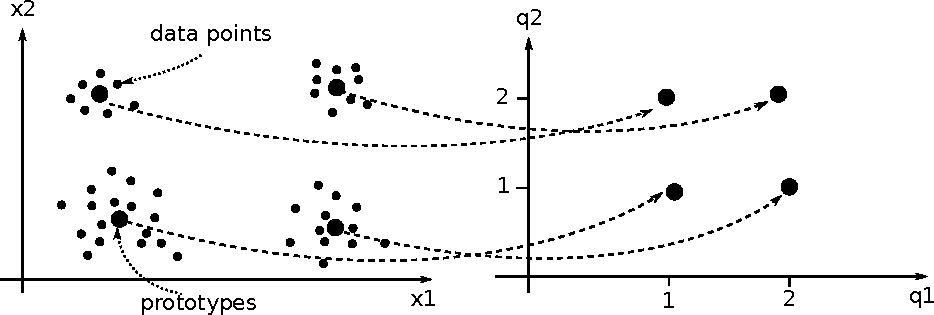
\includegraphics[width=12cm]{section4_fig9}
\end{center}
\[ \text{''map'' of data space} \left\{ \begin{array}{ll}
	\text{visualization} \\\\
	\text{dimension reduction} \\\\
	\text{preprocessing for prediction}
\end{array}\right. \]
\\\\
\paragraph{Notes regarding algorithm \ref{alg:kohonen}} 
\begin{itemize}
\item a common choice to initialise the prototypes is to use the
  data-mean and small vectors $\vec{\eta}_q$ along the first 2 PCs.
\item learning in topographic maps can be understood as a modification
  of the K-means clustering method that breaks permutation symmetry
  $\leadsto$ neighboring neurons should undergo similar changes of
  prototypes during learning
\end{itemize}
\begin{algorithm}
\DontPrintSemicolon  
\textbf{Initialization:} \;
- choose no. $M$ of partitions (``neurons'')\;
- choose annealing schedule for $\varepsilon$ and $\sigma$\;
- initialize prototypes, e.g.:  $\vec{w}_{\vec q} = \vec{x} + \vec{\eta}_{\vec q}$ (faster convergence: center of mass + random in plane of first two principal components) \;
\Begin(){
  choose a data point $\vec{x}^{(\alpha)}$ \\
  determine the closest prototype:
  \[ \vec{p} = \argmin_{\vec r} \big| \vec{x}^{(\alpha)} - 
  \vec{w}_{\vec r}^{\mathrm{old}} \big|
  \]
  change prototypes according to:
  \[ \Delta \vec{w}_{\vec q} = \varepsilon \; h_{\vec{q} \vec{p}} \;
  \big( \vec{x}^{(\alpha)} - \vec{w}_{\vec q}^{\mathrm{old}} \big)
  \]
}
\label{alg:kohonen}
\caption{Online learning for SOMs (Kohonen map) -- ``Vanilla Kohonen''}
\end{algorithm}

\paragraph{Interpretation of the  neighborhood function $h_{\vec{q} \vec{p}}$}
\label{sec:interpr-neighb-funct}
\begin{itemize}
	\item large for neighboring neurons in the neural network
	\item enforces similar learning steps for neighboring neurons
	\item typical choice:
	\begin{equation} \tag{Gauss function}
		h_{\vec{q} \vec{p}} = \exp \bigg\{ - \frac{ (\vec{q}
			- \vec{p} )^2 }{2 \sigma^2} \bigg\}
	\end{equation}
        \itl using $\delta_{\vec{q} \vec{p}}$ as the neighborhood function $h_{\vec{q} \vec{p}}$ in algorithm (\ref{alg:kohonen}) results in standard k-means
      \item \emph{annealing of the parameter $\sigma$:} Start with
        $\sigma$ large ($\leadsto$ neighborhood function convex over
        its support) and decrease linearly or exponentially (but
        ''slow'') during learning. Solution will depend on 
        final value of $\sigma$:
		\begin{itemize}
                  \itr $\sigma = 0$: solution corresponds to a minimum
                  of the K-means clustering cost function (cf.\
                  section \ref{sec:kmeans}) but will be
                  \emph{neighborhood preserving} ($\leadsto$
                  permutation symmetry) \itr $\sigma$ small but
                  finite: better visualization capabilities at the
                  expense of a non-optimal clustering cost
		\end{itemize}
\end{itemize}

\paragraph{Dimension reducing mappings:}\label{sec:dimens-reduc-mapp}
For observations $\vec{x} \in \mathbb{R}^N, N$ typically larger than 
2, 2D Self-Organizing Map can be used for visualization purposes. How this 
reduction of dimensionality is performed is illustrated in figure \ref{fig:som1}
for a 1D example with finite range $\sigma$ of the neighborhood function. 
\begin{figure}
  \centering
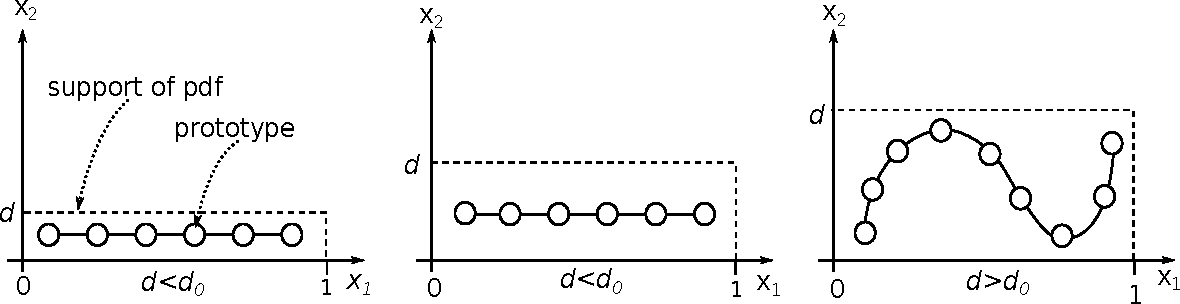
\includegraphics[width=12cm]{section4_fig10}  
  \caption{Dimensionality reduction with SOMs: For small $d$, the one-dimensional topographic map naturally covers variability of the data. For large $d$, the map starts to meander to capture both directions of variability in the data.}
  \label{fig:som1}
\end{figure}

\begin{itemize}
  \itR automatic selection of relevant feature dimension
  \itR hierarchical maps, semantic maps, OR/OD maps 
\slideref{3D surface, Leptograpsus data}
\itR depending on the purpose, number of network units should be chosen small ($\leadsto$ clustering) or large enough ($\leadsto$ visualisation).  
\end{itemize}


% -----------------------------------------------------------------------------

\subsubsection{Self-Organizing Maps for Pairwise Data}
\label{sec:pairwiseSOMs}
\paragraph{Data:} distance matrix $\vec{D}$ specifying the distances or 'dissimilarities' $d_{\alpha \alpha^{'}}$ between a set of $p$ ''objects'' $\alpha, \alpha' = 1, \ldots, p$
\paragraph{Model:} set of $M$ clusters (partitions) $\vec{q}$ with a geometrical
structure (e.g.\ 1-d line or 2-d grid). 
\\\\
binary assignment variables (normalized):
\begin{equation}
	m_{\vec{q}}^{(\alpha)} = \left\{ \begin{array}{ll}
		1, & \text{if object } \alpha \text{ belongs to cluster } \vec q \\\\
		0, & \text{else}
	\end{array} \right.
\end{equation}
cost function:
\begin{equation}
	E_{\big[ \big\{ m_{\vec{q}}^{(\alpha)} \big\} \big]}
	= \frac{1}{p} \sum\limits_{\vec{r}} 
		\frac{ \sum\limits_{\alpha, \alpha^{'}} 
		\Big( \sum\limits_{\vec{q}} 
		\overbrace{h_{\vec{r} \vec{q}}}^{ \substack{\text{neighborhood} \\
		\text{function}}} 
		m_{\vec{q}}^{(\alpha)} \Big) \Big( \sum\limits_{\vec{q}}
		h_{\vec{r} \vec{q}} m_{\vec{q}}^{(\alpha^{'})} \Big)
		d_{\alpha \alpha^{'}} }{
			\sum\limits_{\alpha} \Big( \sum\limits_{\vec{q}}
			h_{\vec{r} \vec{q}} m_{\vec{q}}^{(\alpha)}\Big)}
\end{equation}
\begin{itemize}
      \itl $E$ corresponds to the average cost (min. data pt. distance) of groups that are close by
	\itl replace $m_q^{(\alpha)}$ of pairwise clustering by 
		$\sum\limits_{\vec{q}} h_{\vec{r} \vec{q}} 
		m_{\vec{q}}^{(\alpha)}$
	\itl ''neighboring'' cluster (w.r.t. $h_{\vec{r} \vec{q}}$) contribute
		to the total average distance
	\itl ''neighborhood preserving maps'' induce lower cost
\end{itemize}
model selection
\begin{equation}
	E_{ \big[ \big\{ m_{\vec{q}}^{(\alpha)} \big\} \big] }
	\eqexcl \min
\end{equation}
\textbf{Optimization:} similar to pairwise mean field clustering
(alg.~\ref{alg:meanFieldClustering}), algorithm
\ref{alg:pairwiseMeanFieldSom} implements mean-field annealing to
train SOMs on pairwise data (see \cite{GraepelObermayer1999}).

\begin{algorithm}
\DontPrintSemicolon
\textbf{Initialization:} \;
- choose no. of partitions\;
- choose initial  ($\beta_0$) and final ($\beta_f$) values of the noise parameter\;
- choose annealing factor  $\eta$\;
- choose convergence criterion  $\theta$\;
- initialization of mean-fields  $e_{\vec q}^{(\alpha)}:$ random numbers  $\in [0, 1]$ \;
$\beta \leftarrow \beta_0$\;
\While(annealing){$\beta < \beta_e$}{
\Repeat( EM){ $\big| \big( e_{\vec{q}}^{(\alpha)} \big)_{\mathrm{new}} - \big( e_{\vec{q}}^{(\alpha)} \big)_{\mathrm{old}} \big| < \theta \text{ for all } \vec{q}, \alpha$}{
compute assignment probabilities
\[ \big< m_{\vec{q}}^{(\alpha)} \big>_Q = \frac{ \exp \big\{ -\beta
	\big( e_{\vec{q}}^{(\alpha)} \big)_{\mathrm{old}} \big\}}{
		\sum\limits_r \exp \big\{ -\beta \big( e_{\vec{r}}^{(\alpha)}
		\big)_{\mathrm{old}} \big\} }
	\text{ for all } \vec{q}, \alpha
\]
compute new mean-fields
\[ \begin{array}{lll}
	\big( e_{\vec{q}}^{(\alpha)} \big)_{\mathrm{new}}
	& = &\frac{1}{p} \sum\limits_{\vec{s}} 
		\underbrace{ h_{\vec{s} \vec{q}} }_{ \circledast }
		\Bigg[
		\frac{1}{\sum\limits_{\gamma} \Big( \sum\limits_{\vec{r}}
		h_{\vec{s} \vec{q}} \big< m_{\vec{r}}^{(\gamma)} \big>_Q \Big)}
		\sum\limits_{\delta} \bigg( \sum\limits_{\vec{r}} 
		h_{\vec{s} \vec{r}} \big< m_{\vec{r}}^{(\delta)} \big>_Q \bigg]
		\\\\
	&& \cdot \bigg\{ d_{\delta \alpha} -\frac{1}{2} \frac{1}{
		\sum\limits_{\gamma} \Big( \sum\limits_{\vec{r}} 
		h_{\vec{s} \vec{r}} \big< m_{\vec{r}}^{(\gamma)} \big>_Q \Big)}
		\sum\limits_{\varepsilon} \bigg( \sum\limits_{\vec{r}}
		h_{\vec{s} \vec{r}} \big< m_{\vec{r}}^{(\varepsilon)}
		\big>_Q \bigg) d_{\varepsilon \delta} \bigg\} \Bigg]
		\\\\
	&& \text{for all } \vec{q}, \alpha
\end{array} \]
}
$\beta \leftarrow \eta \beta$\;
}
\label{alg:pairwiseMeanFieldSom}
\caption{Meanfield EM-learning for SOMs with pairwise data}
\end{algorithm}

\paragraph{Comments} \label{sec:comments}
\begin{itemize}
\item replacing $h_{\vec{s} \vec{p}}$ by $\delta_{\vec{s} \vec{p}}$ in algorithm 
\ref{alg:pairwiseMeanFieldSom} recovers standard pairwise clustering (see section
  \ref{sec:generalPairwiseClustering})
\item replacing $h_{\vec{s} \vec{p}}$ by $\delta_{\vec{s} \vec{p}}$
  for the neighborhood function (only) at $\circledast$ in algorithm 
\ref{alg:pairwiseMeanFieldSom} is called
  the ''Kohonen-approximation'' (because the original algorithm
  suggested by T. Kohonen is recovered for squared Euclidean distances
  $d_{\alpha \alpha^{'}}$ and $\beta \rightarrow \infty$)
		\begin{itemize}
			\itr reduction of computational cost
			\itr visualization properties remain
		\end{itemize}
\item no need to anneal $\sigma$ since mean-field annealing (``robust method'')
\end{itemize}
\slideref{noisy spiral, brain connectivity pattern}

% -----------------------------------------------------------------------------

\subsubsection{Euclidean Distances}

observations (feature vectors): $\vec{x}^{(\alpha)}, \alpha = 1, \ldots, p, \vec{x}^{(\alpha)} \in \mathbb{R}^N$
\\\\
distance measure:
\begin{equation}
	d_{\alpha \alpha^{'}}
	= \frac{1}{2} \big( \vec{x}^{(\alpha)} - \vec{x}^{(\alpha^{'})}
		\big)^2
\end{equation}
cost function:
\begin{equation}
	\begin{array}{ll}
	E_{ \big[ \big\{ m_{\vec{q}}^{(\alpha)} \big\} \big] }
	& = \frac{1}{p} \sum\limits_{\vec{q}, \alpha} \Big( 
		\sum\limits_{\vec{p}} h_{\vec{q} \vec{p}} m_{\vec{p}}^{(\alpha)}
		\Big) \big( \vec{x}^{(\alpha)} - \vec{w}_q \big)^2 \\\\
	& = \frac{1}{p} \sum\limits_{\vec{p} \alpha} m_{\vec{p}}^{(\alpha)}
		\sum\limits_{\vec{q}} h_{\vec{q} \vec{p}} \big( 
		\vec{x}^{(\alpha)} - \vec{w}_{\vec{q}} \big)^2 \\\\
	& = E_{ \big[ \big\{ m_{\vec{q}}^{(\alpha)} \big\}, \big\{ 
		\vec{w}_{\vec{q}} \big\} \big] }^T
	\end{array}
\end{equation}
$\corresponds$ K-means cost function, but with a different distance measure:
\begin{equation}
	\sum\limits_q h_{\vec{q} \vec{p}} \big( \vec{x}^{(\alpha)} -
		\vec{w}_{\vec{q}} \big)^2
\end{equation}
instead of: $\big( \vec{x}^{(\alpha)} - \vec{w}_{\vec{p}} \big)^2$
\\\\
where:
\begin{equation}
	\vec{w}_{\vec{q}} 
	= \underbrace{
		\frac{ \sum\limits_{\alpha^{'}} \Big( \sum\limits_{\vec{p}}
		h_{\vec{q} \vec{p}} m_{\vec{p}}^{(\alpha^{'})} \Big) 
		\vec{x}^{(\alpha^{'})} }{ 
			\sum\limits_{\alpha^{'}} \Big(
			\sum\limits_{\vec{p}} h_{\vec{q} \vec{p}}
			m_{\vec{p}}^{(\alpha^{'})} \Big) } }_{
	\substack{	\text{center of mass of all data} \\
			\text{which belongs to cluster } \vec{p}, \\
			\text{weighted by the neigborhood} \\
			\text{function } h_{\vec{q} \vec{p}}}}
\end{equation}
proof: replace $m_q^{(\alpha)}$ by $\sum\limits_{\vec{p}} h_{\vec{q} \vec{p}} m_{\vec{p}}^{(\alpha)}$ in the corresponding derivation in section \ref{sec:pairwiseEuclidean}.
\\\\
\paragraph{On-line Minimization of $E_{ \big[ \big\{ m_q^{(\alpha)}
    \big\}, \big\{ \vec{w}_q \big\} \big] }$:}
Using pairwise squared distances yields a simple on-line version (Algorithm \ref{alg:onlineSOM}) of the learning algorithm for topographic maps. 
\begin{algorithm}
  \DontPrintSemicolon
Initialization of prototypes\;
Select learning step  $\eta$ \;
\Begin(){
choose a data point $\vec{x}^{(\alpha)}$\;
assign data point to the 'closest' prototype\;
\[ \vec{p} = \argmin_{\vec{r}} \sum\limits_{\vec{p}} 
	\underbrace{ h_{\vec{r} \vec{p}} }_{ \circledast }
	\big( \vec{x}^{(\alpha)} - \vec{w}_{\vec{p}}^{\mathrm{old}}
	\big)^2
\]
change all prototypes according to
\[ \Delta \vec{w}_{\vec{q}} = \eta h_{\vec{p} \vec{q}} \big( \vec{x}^{(\alpha)}
	-\vec{w}_{\vec{q}} \big) \text{ for all } \vec{q}
\]
}
\label{alg:onlineSOM}
\caption{Online learning for SOMs and Euclidean distances}
\end{algorithm}
\\\\
\textbf{Comments}
\begin{itemize}
  \item cost-function based approach to the Self-Organizing Map 
  \item $h_{\vec{q} \vec{r}} \rightarrow \delta_{\vec{q} \vec{r}}
  $ at $\circledast$ (see above) is called the Kohonen-approximation
  \item using the Kohonen approximation and Euclidean distance in
  section \ref{sec:pairwiseSOMs} leads to a ''deterministic
  annealing'' version of the standard Self-Organizing Map
\end{itemize}


% -----------------------------------------------------------------------------

\newpage
\subsection{Locally Linear Embedding}
\begin{figure}[h]
	\centering
	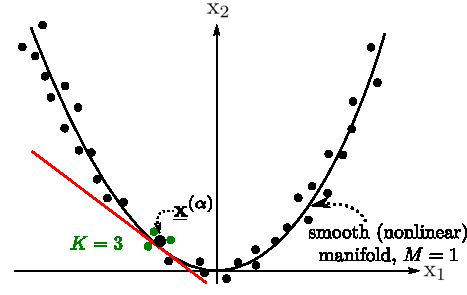
\includegraphics[width=7cm]{section4_fig11.pdf}
\end{figure}
Project the data into the tangential (linear) space of the data manifold.
\begin{wrapfigure}{r}{0.5\textwidth}
  \begin{center}
    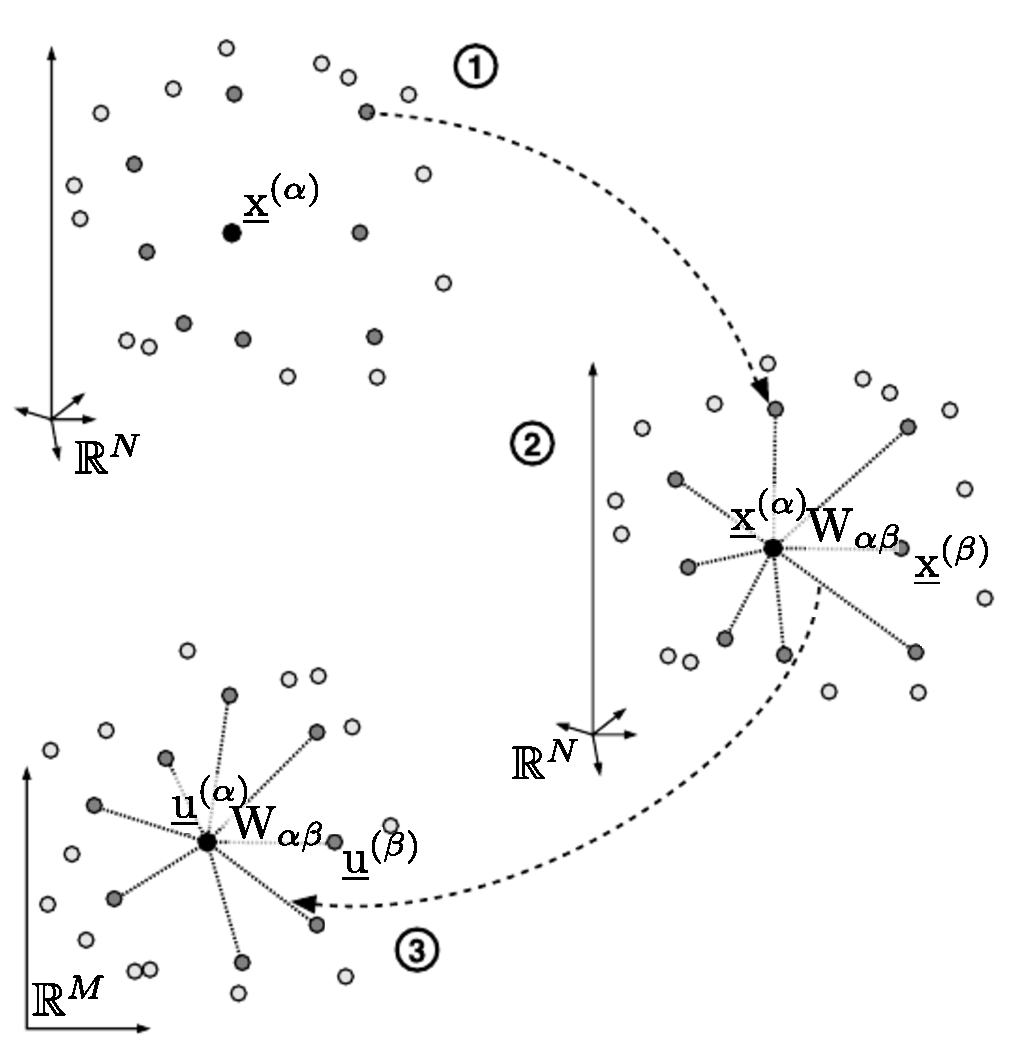
\includegraphics[width=0.3\textwidth]{section4_fig12}
  \end{center}
\end{wrapfigure}
\vspace{-0.2cm}
\begin{itemize}
	\item data points  $\vec{x}^{(\alpha)} \in \mathbb{R}^N$
	\item embedded data points  $\vec{u}^{(\alpha)} \in \mathbb{R}^M, \quad M < N$
\end{itemize}
\small For each data point $\vec{x}^{(\alpha)}$
\begin{itemize}
	\item find the $K$ nearest neighbors
	\item calculate reconstruction weights $\vec{W}$\\ s.t. $\vec{x}^{(\alpha)} \approx \sum_{\beta \in \operatorname{KNN}(\vec{x}^{(\alpha)})}^{} \mathrm{W}_{\alpha \beta} \cdot \vec{x}^{(\beta)}$
	\item obtain embedding $\vec{u}^{(\alpha)} \in \mathbb{R}^M$\\ s.t. $\vec{u}^{(\alpha)} \approx \sum_{\beta \in \operatorname{KNN}(\vec{x}^{(\alpha)})}^{} \mathrm{W}_{\alpha \beta} \cdot \vec{u}^{(\beta)}$
\end{itemize}

\paragraph{Step 1: find $K$ nearest neighbors}
choice: Euclidean distance
\begin{eqnarray*}
	\beta_1^{(\alpha)} &=& \arg \min_{\mathrlap{\beta}} \qquad \abs{\vec{x}^{(\alpha)} - \vec{x}^{(\beta)}} \\
	\beta_2^{(\alpha)} &=& \arg \min_{\mathrlap{\beta \neq \beta_1^{(\alpha)}}} \qquad \abs{\vec{x}^{(\alpha)} - \vec{x}^{(\beta)}} \\
	\vdots &&\\
	\beta_K^{(\alpha)} &=& \arg \min_{\mathrlap{\beta \neq \beta_1^{(\alpha)},k=1, \dots, K-1}} \qquad \abs{\vec{x}^{(\alpha)} - \vec{x}^{(\beta)}}\\
	\operatorname{KNN}(\vec{x}^{(\alpha)}) &=& \left\{ \beta_1^{(\alpha)}, \beta_2^{(\alpha)}, \dots, \beta_K^{(\alpha)}  \right\} \qquad \text{(not necessarily unique)}
\end{eqnarray*}
linear data structure (e.g. data matrix): \quad $\mathcal{O}(Np^2)$\\
k-d tree (balanced search tree): \hspace{1.55cm} $\mathcal{O}(Np \log p)$
\newcommand\mydots{\hbox to 1em{.\hss.\hss.}}
\paragraph{Step 2: calculate reconstruction weights}\mbox{}\\
\small
minimize cost function:
\vspace{-0.2cm}
\begin{align*}
E(\vec{W}) = \sum_{\alpha=1}^{p} \underbrace{\abs{\vec{x}^{(\alpha)} - \sum_{\beta=1}^{p} \mathrm{W}_{\alpha \beta} \vec{x}^{(\beta)}}^2}_{\substack{\text{reconstruct } \vec{x}^{(\alpha)} \text{ by its } \\ K \text{ nearest neighbors only}}} \eqexcl \min \quad \text{s.t.} \quad &\mathrm{W}_{\alpha \beta} = 0 \text{ if } \beta \notin \operatorname{KNN}(\vec{x}^{(\alpha)}), \\[-40pt]
&\sum_{\beta=1}^{p} \mathrm{W}_{\alpha \beta} = 1
\end{align*}\\
\vspace{0.2cm}
weight matrix $\vec{W}$: 
\begin{itemize}
	\item sparse: (up to) $K$ nonzero elements per row
	\item not symmetric: nearest neighbors of a data point can have closer neighbors
\end{itemize}
optimal weights are invariant to:
\begin{itemize}
	\item rotation $\vec{R}: \hspace{0.8cm} E\left[ \vec{R}\cdot\vec{x}^{(1)}, \mydots, \vec{R}\cdot\vec{x}^{(p)} \right] \stackrel{\text{orthog. } \vec{R}}{=} E\left[ \vec{x}^{(1)}, \mydots, \vec{x}^{(p)} \right] $ 
	\item scaling $\gamma > 0: \hspace{4.3mm} E\left[ \gamma\vec{x}^{(1)}, \mydots, \gamma\vec{x}^{(p)} \right] = \gamma^2 E\left[ \vec{x}^{(1)}, \mydots, \vec{x}^{(p)} \right]$
	\item translation $\Delta \vec{x}: \hspace{2mm} E\left[ \vec{x}^{(1)}+\Delta \vec{x}, \mydots, \vec{x}^{(p)}+\Delta \vec{x} \right] \stackrel{\sum_{\beta} \mathrm{W}_{\alpha \beta} = 1}{=} E\left[ \vec{x}^{(1)}, \mydots, \vec{x}^{(p)} \right]$
\end{itemize}
for each data point $\vec{x}^{(\alpha)}:$
\begin{itemize}
	\item local ''covariance'' matrix (symmetric \& positive semidefinite) $\vec{C}^{(\alpha)} \in \mathbb{R}^{K,K}:$ 
	\vspace{-0.2cm}
	\begin{equation*}
		\mathrm{C}_{jk} = \big( \vec{x}^{(\alpha)} - \vec{x}^{(\beta_j^{(\alpha)})} \big)^T\big( \vec{x}^{(\alpha)} - \vec{x}^{(\beta_k^{(\alpha)})} \big)
	\end{equation*} 
	\vspace{-0.5cm}
	\item solve linear system $\vec{C}^{(\alpha)}\widetilde{\vec{w}}^{(\alpha)} = (1, \mydots, 1)^T$
	\item rescale weights: $\mathrm{W}_{\alpha \beta_j^{(\alpha)}} = \widetilde{\mathrm{w}}_j^{(\alpha)} / \sum_{k=1}^{K} \widetilde{\mathrm{w}}_k^{(\alpha)}$ to fulfill constraint
\end{itemize}
\vspace{-0.2cm}
$\Rightarrow \vec{W}$ contains the optimal weights with $\mathrm{W}_{\alpha \beta} = 0$ for $\beta \notin \operatorname{KNN}(\vec{x}^{(\alpha)})$ \\\vspace{0.1cm}
$\Rightarrow p$ dense $K$-dim. linear systems have to be solved: \quad $\mathcal{O}(pK^3)$ 

\paragraph{Step 3: obtain embedding coordinates}
For any $M$-dimensional manifold there exist linear mappings of each local ''patch'' onto $M$-dimensional coordinates in a linear space
\begin{itemize}
	\item linear mapping: rotation, scaling, translation
	\item weights $\vec{W}$ can be used to optimally reconstruct the data points in the lower-dimensional embedding space
\end{itemize}
idea:
\begin{itemize}
	\item cut $N$-d manifold into small patches
	\item ''glue'' them together in $M$-d using only rotation, scaling, translation for each patch
\end{itemize}
given $M \ll N$ and $\vec{W}:$ find optimal coordinates $\underbrace{\vec{u}^{(1)}, \mydots, \vec{u}^{(p)}}_{=\vec{U} \in \mathbb{R}^{M,p}} \in \mathbb{R}^M$ \\
cost function: 
\begin{equation*}
F(\vec{U}) = \sum_{\alpha=1}^{p} \abs{\vec{u}^{(\alpha)} - \sum_{\beta=1}^{p} \mathrm{W}_{\alpha \beta} \vec{u}^{(\beta)}}^2
\end{equation*}
equivalent quadratic form: 
\vspace{-0.4cm}
\begin{equation*}
F(\vec{U}) = \sum_{\alpha, \beta=1}^{p} g_{\alpha \beta} (\vec{u}^{(\alpha)})^T \vec{u}^{(\beta)}
\end{equation*}

\vspace{-1.2cm}
\begin{flalign*}
\text{where } g_{\alpha \beta} &= \\[-2pt] &\text{\textbf{see blackboard}}  \\[-9pt] &= \delta_{\alpha \beta} - \mathrm{W}_{\alpha \beta} - \mathrm{W}_{\beta \alpha} + \sum_{\gamma=1}^{p} \mathrm{W}_{\gamma \alpha} \mathrm{W}_{\gamma \beta} \hspace{4cm}
\end{flalign*}
$\vec{G} = \left\{ g_{\alpha \beta} \right\} \in \mathbb{R}^{p,p}$ is symmetric and positive semidefinite\\
minimize cost function:
\begin{equation*}
F(\vec{U}) = \sum_{\alpha, \beta=1}^{p} g_{\alpha \beta} (\vec{u}^{(\alpha)})^T \vec{u}^{(\beta)}
\end{equation*}
 \vspace{-0.5cm}
\begin{align*}
\quad \text{s.t.} \quad &\sum_{\alpha=1}^{p} \vec{u}^{(\alpha)} = 0,\quad \text{(remove translation freedom)} \\
&\frac{1}{p} \sum_{\alpha=1}^{p} \vec{u}^{(\alpha)} (\vec{u}^{(\alpha)})^T = \vec{I} \quad \text{(prevent trivial solutions e.g., } \vec{u}^{(\alpha)} = \vec{0})
\end{align*}

\begin{itemize}
	\itl w.l.o.g. as $F(\vec{U})$ invariant to rotation, scaling, translation
	\itl implies that reconstruction errors for different coordinates are measured on the same scale
\end{itemize}
\newcommand{\myvdots}{\raisebox{3pt}{\scalebox{.75}{\vdots}}}

\paragraph{Step 3: obtain embedding coordinates}
\vspace{-0.3cm}
solution: \\\vspace{0.2cm}
compute the $M+1$ eigenvectors of $\vec{G}$ with the lowest eigenvalues but discard the eigenvector $\vec{e}_p = \frac{1}{p} (1, \mydots, 1)^T$ with eigenvalue 0 (corresponding to translation) 
\vspace{-0.2cm}
\begin{equation*}
\vec{U} = \begin{pmatrix}
\vec{e}_{p-M}^T \\ \myvdots \\ \vec{e}_{p-1}^T
\end{pmatrix} = \left(\vec{u}^{(1)}, \mydots, \vec{u}^{(p)}\right) \quad \text{(solution satisfies both constraints)}
\end{equation*}
implementation:
\begin{itemize}
	\item store $\vec{W}$ in sparse matrix format (at most $K \cdot p$ non-zero elements) and calculate $\vec{G} = \Big( \vec{I} - \vec{W}^T \Big) \Big( \vec{I} - \vec{W} \Big) \in \mathbb{R}^{p,p}$ 
	\item use sparse eigenvalue solvers (eigsh) \\\vspace{0.1cm}$\vec{v} \mapsto \vec{G} \cdot \vec{v} = \Big( \vec{I} - \vec{W}^T \Big) \Big[ \Big( \vec{I} - \vec{W} \Big) \vec{v} \Big]$
\end{itemize}
\slideref{Ex: LLE vs PCA for human faces translated in 2D}
\paragraph{Summary of the LLE algorithm}\mbox{}\\
parameters: $K,M$
\begin{enumerate}
	\item find $K$ nearest neighbors $\operatorname{KNN}(\vec{x}^{(\alpha)}) = \left\{ \beta_1^{(\alpha)}, \mydots, \beta_K^{(\alpha)} \right\}$ $\forall \alpha=1, \mydots, p$
	\item calculate (locally invariant) reconstruction weights $\vec{W}$:
\end{enumerate}
\vspace{-0.1cm}
\begin{align*}
\vec{C}^{(\alpha)}\widetilde{\vec{w}}^{(\alpha)} &= (1, \mydots, 1)^T, \quad \forall \alpha=1, \mydots, p \\
\mathrm{W}_{\alpha \beta_j^{(\alpha)}} &= \frac{\widetilde{\mathrm{w}}_j^{(\alpha)}}{\sum_{k=1}^{K} \widetilde{\mathrm{w}}_k^{(\alpha)}}
\end{align*}
\vspace{-0.2cm}
\begin{enumerate}
	\setcounter{enumi}{2}
	\item calculate the embedding coordinates $\vec{U}$: \\\vspace{0.1cm}
	compute the $M+1$ eigenvectors $\left( \vec{e}_p, \mydots, \vec{e}_{p-M} \right)$ of  $\vec{G}$ \\with the smallest eigenvalues
\end{enumerate}
\vspace{-0.2cm}
\begin{align*}
 g_{\alpha \beta} &= \delta_{\alpha \beta} - \mathrm{W}_{\alpha \beta} - \mathrm{W}_{\beta \alpha} + \sum_{\gamma=1}^{p} \mathrm{W}_{\gamma \alpha} \mathrm{W}_{\gamma \beta} 
\end{align*}
\vspace{-0.2cm}
\begin{align*}
 \vec{G} \cdot \vec{e}_j = \lambda_j \vec{e}_j \hspace{2cm}
\vec{U} = \begin{pmatrix}
\vec{e}_{p-M}^T \\ \myvdots \\ \vec{e}_{p-1}^T
\end{pmatrix} = \left(\vec{u}^{(1)}, \mydots, \vec{u}^{(p)}\right)
\end{align*}

\paragraph{Remarks}
\small
\begin{itemize}
	\item efficient \& robust algorithm
	\vspace{0.2cm}
	\item parameters: number $K$ of neighbors, embedding dimension $M$
	\vspace{0.2cm}
	\item convex optimization problem, standard (sparse) linear algebra methods suffice 
	\vspace{0.2cm}
	\item for $K > N$ regularization is required (singular covariance matrix $\vec{C}^{(\alpha)}$)
	\vspace{-0.1cm}
	\begin{equation*}
		\vec{C}^{(\alpha)} \leftarrow \vec{C}^{(\alpha)} + \varepsilon \vec{I}
	\end{equation*} 
	\vspace{-0.7cm}
	\item extension for pairwise data available via non-Euclidean distances $d_{\alpha \alpha'}$ in $\vec{C}^{(\alpha)}$
	\vspace{0.2cm}
	\item alternative methods available (e.g. Laplacian eigenmaps, t-stochastic neighbor embedding, isomap, Kernel PCA)
\end{itemize}
